\documentclass[border=4pt,tikz]{standalone}
\usepackage[utf8]{inputenc}
\usepackage[T1]{fontenc}
\usepackage{tikz}
\usepackage{xcolor}
\usetikzlibrary{positioning, shapes.geometric, arrows.meta, calc}
\definecolor{nodeFill}{HTML}{E8EEF7}
\definecolor{nodeStroke}{HTML}{1F3A5F}
\definecolor{accent}{HTML}{3D5A80}
\definecolor{textDark}{HTML}{1A1A1A}
\begin{document}
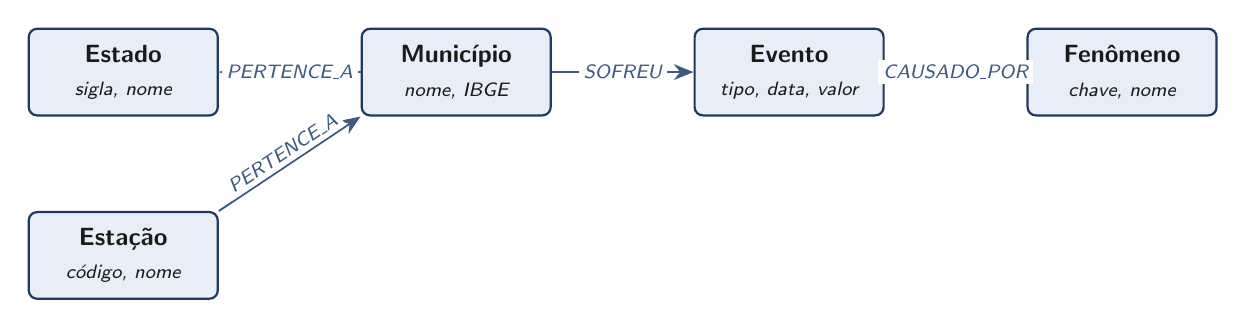
\begin{tikzpicture}[
  font=\sffamily\small,
  every node/.style={text=textDark},
  entity/.style={
    rectangle, rounded corners=3pt,
    draw=nodeStroke, line width=0.8pt,
    fill=nodeFill,
    minimum width=24mm, minimum height=11mm,
    align=center, inner sep=3pt
  },
  rel/.style={
    -{Stealth[length=2.5mm, width=2mm]},
    draw=accent, line width=0.7pt
  },
  rellabel/.style={
    font=\sffamily\scriptsize\itshape,
    text=accent, fill=white, inner sep=1.8pt
  }
]
  \node[entity] (estado) {\textbf{Estado}\\[1pt]\scriptsize\itshape sigla, nome};
  \node[entity, right=18mm of estado]  (municipio) {\textbf{Município}\\[1pt]\scriptsize\itshape nome, IBGE};
  \node[entity, right=18mm of municipio] (evento)  {\textbf{Evento}\\[1pt]\scriptsize\itshape tipo, data, valor};
  \node[entity, right=18mm of evento]    (fenomeno) {\textbf{Fenômeno}\\[1pt]\scriptsize\itshape chave, nome};
  \node[entity, below=12mm of estado] (estacao) {\textbf{Estação}\\[1pt]\scriptsize\itshape código, nome};

  \draw[rel] (municipio) -- (estado)
    node[rellabel, midway] {PERTENCE\_A};
  \draw[rel] (municipio) -- (evento)
    node[rellabel, midway] {SOFREU};
  \draw[rel] (evento) -- (fenomeno)
    node[rellabel, midway] {CAUSADO\_POR};
  \draw[rel] (estacao.north east) -- (municipio.south west)
    node[rellabel, midway, sloped, above] {PERTENCE\_A};
\end{tikzpicture}
\end{document}
